\documentclass[a4paper]{article}
\usepackage[margin=2cm]{geometry}

\usepackage{fontspec}
\usepackage{animate}
\usepackage{graphicx}
\usepackage[catalan]{babel}
\usepackage{hyperref}
\usepackage{float}
\usepackage{array}
\usepackage[table, dvipsnames]{xcolor}

\hypersetup{
	colorlinks = true,
	linkcolor = black,
	urlcolor = blue,
}

\setlength{\parindent}{0pt}
\setlength{\parskip}{0.2cm}

\begin{document}
\begin{titlepage}
	\centering
	\vspace{1cm}
	
\includegraphics[width=0.25\textwidth]{images/etseib}
	\par\vspace{1cm}
	\textsc{ \LARGE Escola Tècnica Superior d'Enginyeria \\[1em] 
		Industrial de Barcelona}
	\par\vspace{2cm}
	\textbf{\Huge Tècniques Estadístiques per la Qualitat}
	\par\vspace{2cm}
	{\LARGE Informe pràctiques}
	\vfill
	\begin{flushright}
		\large
		Marc Asenjo i Ponce de León \par
		Joan Marcè i Igual \par
		Iñigo Moreno i Caireta \par
		Esteve Tarragó Sanchís \par
	\end{flushright}
\end{titlepage}

\tableofcontents
\pagebreak

\section{Introducció}
En aquest treball s'han usat les tècniques de disseny d'experiments per poder veure el funcionament d'un sistema. Per tal de poder tenir una motivació més alta, s'ha contactat amb l'empresa \emph{\href{http://www.protein.es/}{Proteïn S.A.}} de manera que el cas presentat fos un real. 

\subsection{Tema escollit}
L'activitat principal de \emph{Proteïn S.A.} és fabricar  \emph{\href{https://es.wikipedia.org/wiki/Col\%C3\%A1geno_hidrolizado}{co\l.lagen hidrolitzat}} a partir de l'ós de porc que és usat a la indústria de l'alimentació per afegir els nutrients necessaris a la carn. 

A part, un subproducte que es genera és el \emph{\href{https://es.wikipedia.org/wiki/Fosfato_tric\%C3\%A1lcico}{Fosfat Tricàlcic}} ($Ca_3 (PO_4)_2$) o també conegut com \emph{apatita} i un dels usos més comuns és per les gallines que ponen ous perquè no es quedin sense calci.

El problema principal de l'apatita és que els compradors la volen amb un \% en massa igual o superior al 15\%. Si aquesta condició no es pot garantir els clients reclamaran indemnitzacions o aniran a comprar a la competència. Així doncs, aquest serà l'objecte principal de l'estudi ja que l'empresa vol assegurar-se que la qualitat de la seva apatita és bona. 

A part també hi ha co\l.lagen que s'escapa per la línia de l'apatita a l'hora de separar els dos productes pel que també pot ser d'interès minimitzar la quantitat que es perd perquè no s'ha pogut separar prou bé.

\subsection{Objectius}
Donat que els clients poden reclamar si la qualitat d'apatita no és suficient i que hi ha part de co\l.lagen que es perd per la línia de l'apatita ens interessa complir els següents objectius:

\begin{itemize}
	\item Maximitzar el \% en massa d'apatita
	\item Minimitzar el \% en massa de co\l.lagen a la línia de l'apatita
\end{itemize}

\section{Disseny}

\subsection{Sistema a estudiar}
Per poder saber quins factors s'han de controlar cal entendre primer com funciona la part del procés amb el que s'obté l'apatita, veure \autoref{fig:esquema}. Inicialment el producte arriba del procés anterior i conté co\l.lagen i apatita en suspensió en aigua (línia blava al P\&D). Així doncs, s'ha de separar l'apatita de l'aigua, el problema és que precipita molt fàcilment i s'ha de forçar que es mantingui en suspensió. Per tant, hi ha una sèrie d'elements que asseguren que això sigui així; al dipòsit on va a parar (C-03) hi ha un parell de barrejadors i una bomba de recirculació (P-C32). 

\begin{figure}[H]
	\centering
	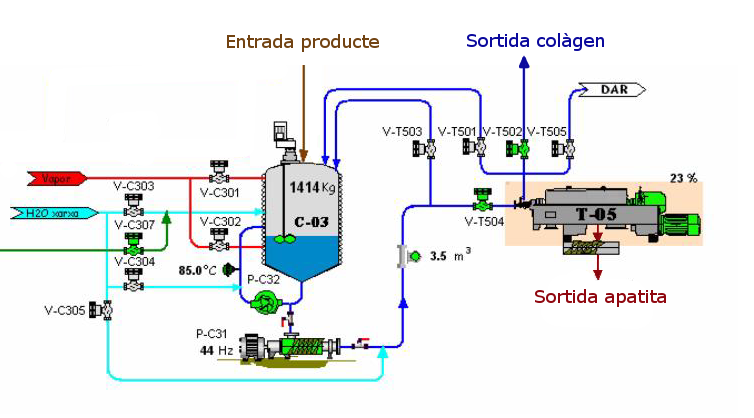
\includegraphics[width=0.8\textwidth]{images/esquema}
	\caption{Esquema del sistema a estudiar}
	\label{fig:esquema}
\end{figure}

Per tal de separar el co\l.lagen i l'apatita s'usa un \emph{\href{https://youtu.be/uvWcLZWM_JY}{tricànter}} (veure \autoref{fig:tricanter}), tot i que en aquest procés només funciona com a \emph{decànter}. Aquesta màquina el que fa és, mitjançant força centrífuga separar els sòlids dels líquids dels greixos, no hi ha greix en aquest cas. Cal tenir en compte que aquesta separació no és perfecte i que part del co\l.lagen s'escapa junt amb l'apatita que s'obté.

Per fer la separació la màquina consta d'un cilindre exterior que gira a alta velocitat i un vis sens fi interior que gira a una mica més ràpid que l'exterior, de manera que el vis sens fi va desplaçant lentament el sòlid cap al final del tricànter, situat a l'esquerra de la \autoref{fig:tricanter}, i el líquid cap al principi. 

Aquesta diferència de velocitats entre els cilindres interiors i exteriors influeix en la velocitat a la que s'elimina el sòlid de dins de la màquina i també en la quantitat d'aigua que contindrà.

\begin{figure}[H]
	\centering
	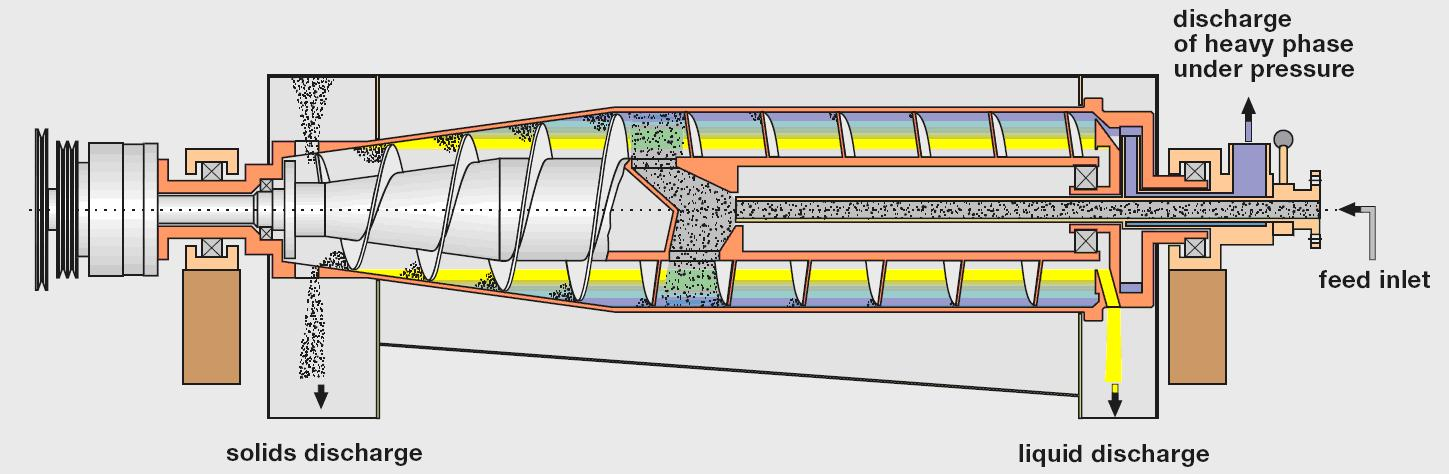
\includegraphics[width=0.8\textwidth]{images/tricanter}
	\caption{Esquema d'un tricànter}
	\label{fig:tricanter}
\end{figure}

\begin{figure}[H]
	\centering
	\animategraphics[draft, autoplay, loop, poster =234, width = 0.5\textwidth]{15}{images/tricanter-movie/tricanter-movie-}{0}{384}
	\caption{Animació explicativa de com funciona un tricanter}
\end{figure}

\subsection{Obtenció i mesura d'una mostra}
Per obtenir una mostra simplement s'agafa de la sortida del tricànter una mica de producte i després es porta al laboratori on es mesurarà.

El procés de mesura és una mica més complicat i consta d'una sèrie d'etapes:

\begin{enumerate}
	\item Es pesa la mostra que conté, entre d'altres, aigua, co\l.lagen i fosfat.
	\item Es posa en un forn a 100ºC per tal d'evaporar tota l'aigua 
	\item Es torna a pesar i es pot veure la quantitat d'aigua que s'ha eliminat
	\item Es posa de nou en un forn però ara a 400ºC per tal d'eliminar mitjançant piròlisi tota la matèria orgànica.
	\item Es torna a pesar i així es pot veure per composició estequiomètrica la quantitat d'apatita en \% en massa que hi havia a la mostra presa.
\end{enumerate} 

\subsection{Factors i nivells}

Un cop s'ha vist el sistema que a estudiar es poden veure els factors que s'hauran de controlar per tal de realitzar l'estudi:

\begin{itemize}
	\item Diferència de velocitats entre els cilindres interior i exterior
	\item Cabal d'entrada al tricànter T-05 (L/h)
	\item Velocitat de la bomba P-C32 (en Hz)
	\item Volum al dipòsit C-03 (en kg)
\end{itemize}

\begin{table}[H]
	\centering
	\renewcommand{\arraystretch}{1.5}
	\rowcolors{2}{gray!25}{white}
	\begin{tabular}{llrr}
		\rowcolor{gray!40}
		Variable Minitab & Factor & Nivell baix & Nivell alt \\
		A & Diferencial & 8 & 12 \\
		B & Cabal H20 (L/h)& 1800 & 2400 \\
		C & Velocitat P-C32 (Hz) & 50 & 75 \\
		D & Volum C-03 (kg) & 1600 & 2000 \\
	\end{tabular}
\end{table}

\subsection{Nombre d'experiments i restriccions externes}
Per tal de realitzar els experiments s'ha decidit amb l'empresa de prendre una mostra cada 12 hores. Aquest interval s'ha decidit així per assegurar-se que el sistema està en equilibri a l'hora de prendre una mostra i que no hi ha altres factors que alteren el resultat, ja que si el sistema es trobés en un estat transitori el resultat es podria veure afectar i això no interessa.

Amb aquest interval de 12 hores entre mostres es calcula que es podran realitzar tots els experiments d'un disseny factorial complet $2^4$ començant a prendre les mostres el 24 de novembre de 2016 i havent acabat als voltants del 16 de desembre de 2016. Tenint en compte que a la fabrica hi poden haver averies o altres incidents que impedeixin realitzar l'experiment.


\end{document}